\documentclass{article}
\usepackage[utf8]{inputenc}
\usepackage{dsfont}
\usepackage{float}
\usepackage{amsmath}
\usepackage{graphicx}
\usepackage[colorinlistoftodos]{todonotes}
\usepackage[colorlinks=true, allcolors=blue]{hyperref}
\usepackage{algpseudocode}
\usepackage{algorithm}

\title{Métodos Constructivos}
\author{Camilo Andrés Rodríguez Garzón}

\author{Camilo Andrés Rodríguez Garzón}
\date{\today}

\begin{document}
\maketitle

\section{Descripción}
En el presente trabajo se desea resolver el problema del viajante. Para esto, se elaboró dos métodos constructivos que permitiecen obtener una ruta y de esta manera resolver dicho problema. Para este trabajo se eligieron el método del vecino más cercano y un método creado y basado en el método pilot (url con implementación de los métodos \href{https://github.com/camilorodriguezga/Tsp}{Tsp}
). A continuación se presenta el algoritmo correspondiente a cada uno de los métodos:

\begin{algorithm}[H]
	\caption{Greedy Tsp}\label{GreedyTsp}
	\begin{algorithmic}[1]
		\Procedure{Build Route}{nameFile}
		\State $coor \gets ReadInput(nameFile)$ \Comment{obtener las coordenadas del archivo}
		\State $coorR \gets coor.pop(0)$ \Comment{se obtiene la primera coordenada y se elimina de la lista}
		\State $dt \gets 0$ \Comment{distancia total en 0}
		\While{$coor$}%\Comment{We have the answer if r is 0}
		\State $d, p_2 \gets NearestNeighbors(coor[length - 1])$ \Comment{se obtiene las coordenadas del vecino más cercano y su distancia}
		\State $coor.remove(p_2)$ \Comment{se remueve la coordenada $p_2$ de la lista}
		\State $dt \gets dt + d$
		\State $coorR.append(p_2)$
		\EndWhile\label{euclidendwhile}
		\State $coorR.append(coorR[0])$ \Comment{se une punto final con inicial}
		\State $drawTsp(coorR.x, coorR.y, dt)$
		\EndProcedure
	\end{algorithmic}
\end{algorithm}

\begin{algorithm}[H]
	\caption{Semi-Pilot Tsp}\label{SemiPilotTsp}
	\begin{algorithmic}[1]
		\Procedure{Build Route}{nameFile, breadth, pilot}
		\State $coor \gets ReadInput(nameFile)$ \Comment{obtener las coordenadas del archivo}
		\State $coorR \gets coor.pop(0)$ \Comment{se obtiene la primera coordenada y se elimina de la lista}
		\State $dt \gets 0$ \Comment{distancia total en 0}
		\State $coorBase \gets copy(coor)$ \Comment{se hace una copia de las coordenadas}
		\State $buildPilot(coorBase, pilot)$ \Comment{se construye pilot y se finaliza ruta con nearest neighbors}
		\State $dt \gets dt + getDistance(coorR[length - 1], coorR[0])$ \Comment{se obtiene distancia final}
		\State $coorR.append(coorR[0])$ \Comment{se une punto final con inicial}
		\State $drawTsp(coorR.x, coorR.y, dt)$
		\EndProcedure
		\\
		\Procedure{Build Pilot}{root, pilot, breadth}
			\State $root.children \gets []$
			\If {$pilot \ge 1$} \Comment{caso cuando es usado el método pilot}
				\State $root.children \gets addChild(root, breadth)$
				\State $pilot \gets pilot - 1$
			\Else \Comment{caso cuando se termina de completar la ruta}
				\State $root.children \gets addChild(root, 1)$
			\EndIf
			\If {root.children is not empty} 
				\For {child in root.children}
					\State buildPilot(child, pilot, breadth)
				\EndFor
			\Else \Comment{cuando la construcción de la ruta es terminada}
				\If {$dt == 0 \ or \ dt > root.d$} \Comment{se guarda la mejor ruta}
					\State $dt \gets root.d$
					\While {root}
						\State coorR.insert(0,root.value) \Comment{se inserta en la lista resultante en la primera posición las coordenadas}
						\State root = root.parent
					\EndWhile
				\EndIf
			\EndIf
		\EndProcedure
	\end{algorithmic}
\end{algorithm}

Se eligió dichos métodos y esto se resume al hecho de aprender en un ambiente más real cuales son las dificultades de implementarlos así como también de adquirir la experiencia de poder construir cada unos de estos.

\section{Resultados}

\subsection{Datos pr439}

\begin{figure}[H]
	\begin{minipage}{0.5\textwidth}
		\centering
		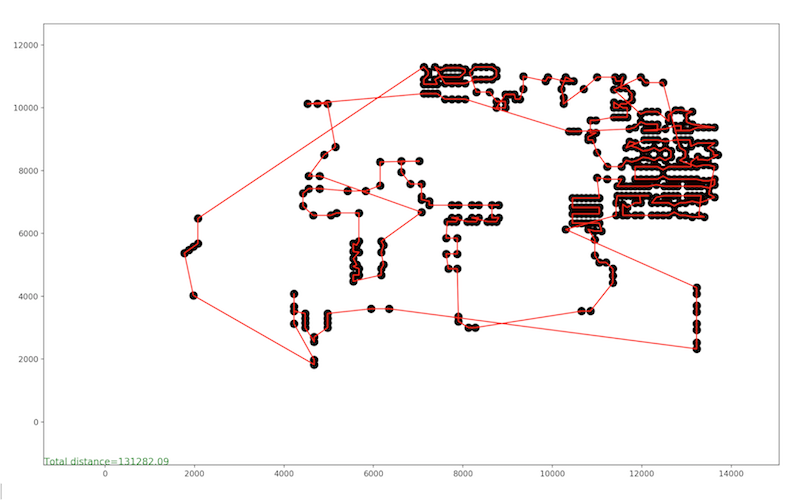
\includegraphics[width=1\textwidth]{../image/greedy/greedy-pr439.png}
		\caption{\label{fig:Figura1} Tsp greedy data pr439}
	\end{minipage}\hfill
	\begin {minipage}{0.5\textwidth}
		\centering
		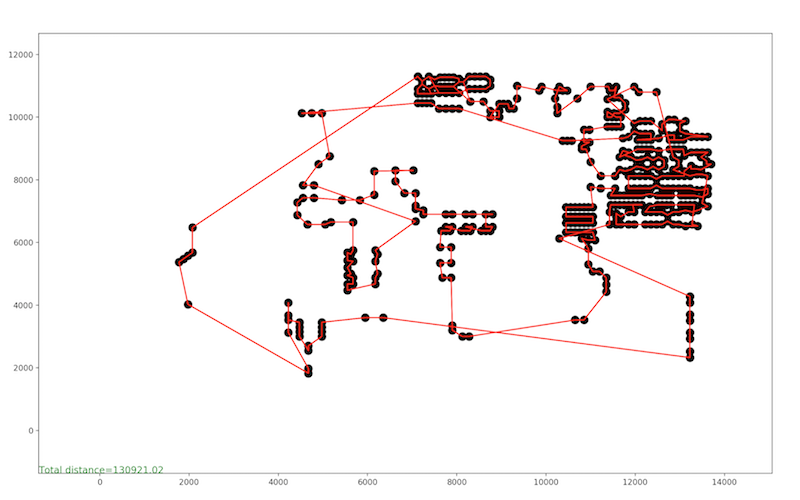
\includegraphics[width=1\textwidth]{../image/semipilot/semipilot-pr439-2-2.png}
		\caption{\label{fig:Figura1} Tsp semipilot data pr439}
	\end{minipage}
\end{figure}

\begin{table}[H]
\centering
\caption{Comparativa de tiempo de ejecución y distancia recorrida de Algoritmos para pr439}
\label{Table:pr439}
\begin{tabular}{| l | l | l | l |}
\hline
Algoritmo & Tiempo Inicial & Tiempo final & Distancia \\ \hline
Vecino más cercano & 2018-03-05 23:15:40.434047 & 2018-03-05 23:15:40.813967 & 131282.09 \\ \hline
Semi-pilot & 2018-03-05 23:11:56.054095 & 2018-03-05 23:11:56.874281 & 130921.02 \\ \hline
TSPLIB & - & - & 107217 \\ \hline

\end{tabular}
\end{table}

\subsection{Datos linhp318}

\begin{figure}[H]
	\begin{minipage}{0.5\textwidth}
		\centering
		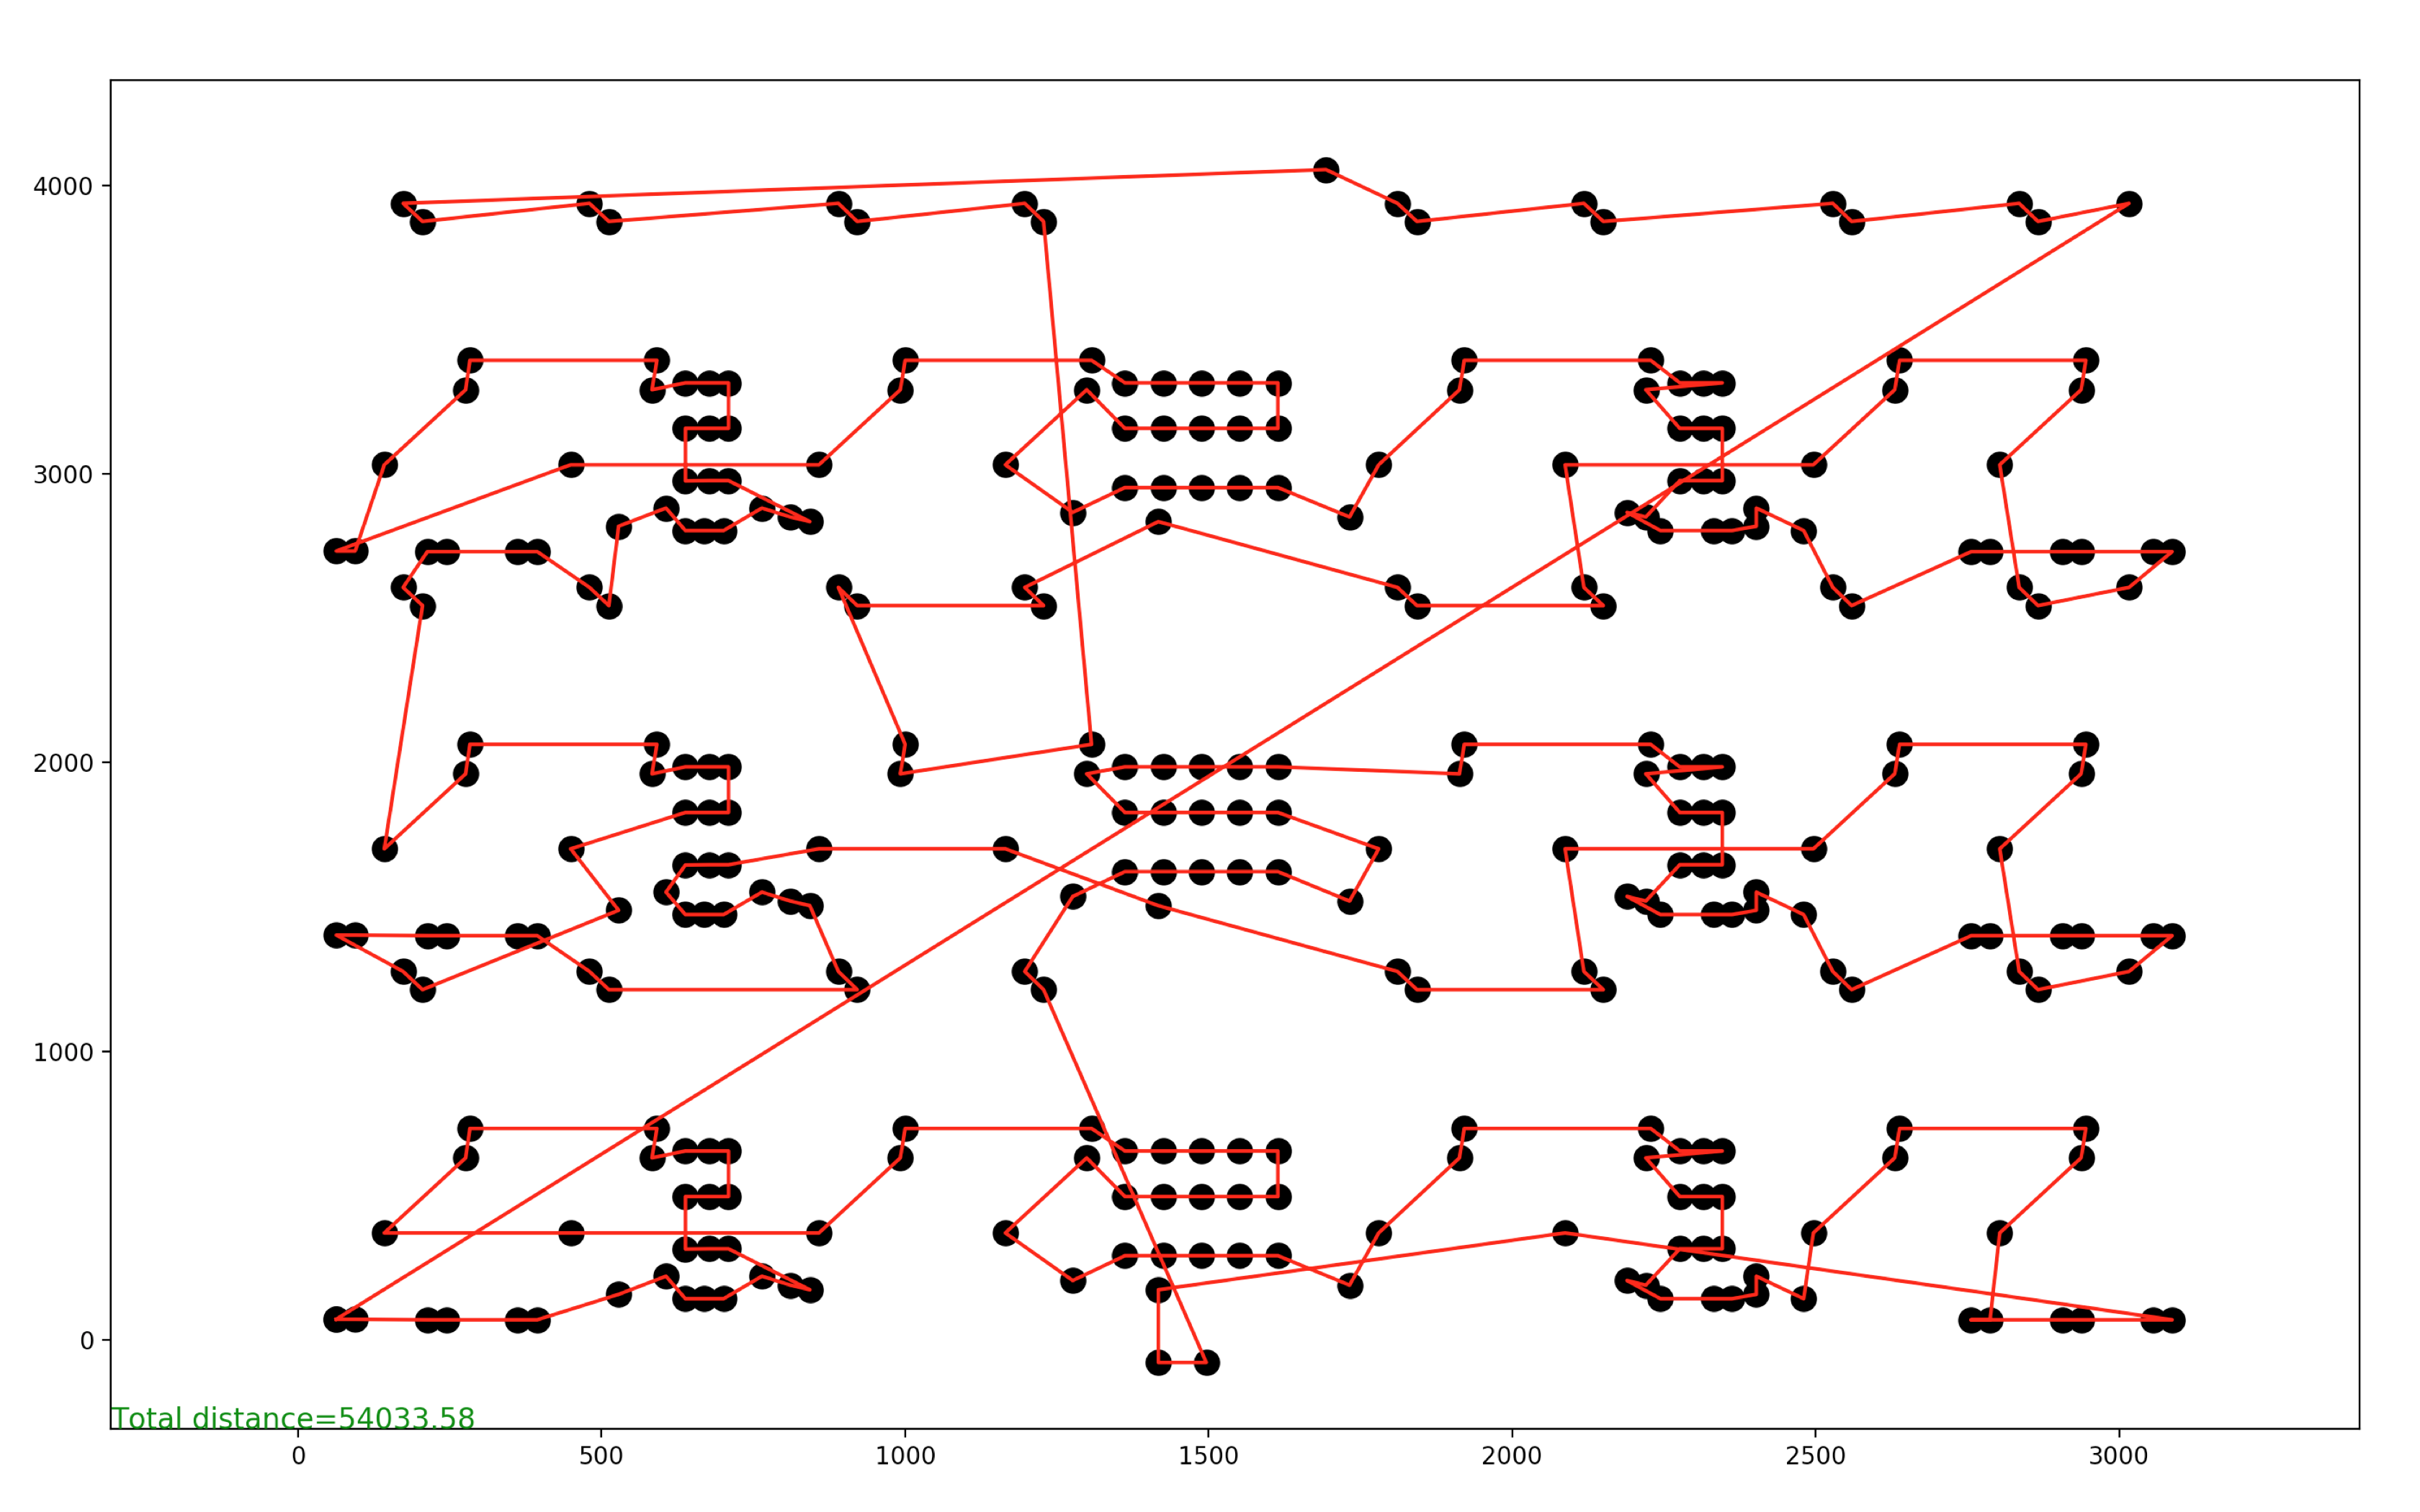
\includegraphics[width=1\textwidth]{../image/greedy/greedy-linhp318.png}
		\caption{\label{fig:Figura1} Tsp greedy data linhp318}
	\end{minipage}\hfill
	\begin {minipage}{0.5\textwidth}
		\centering
		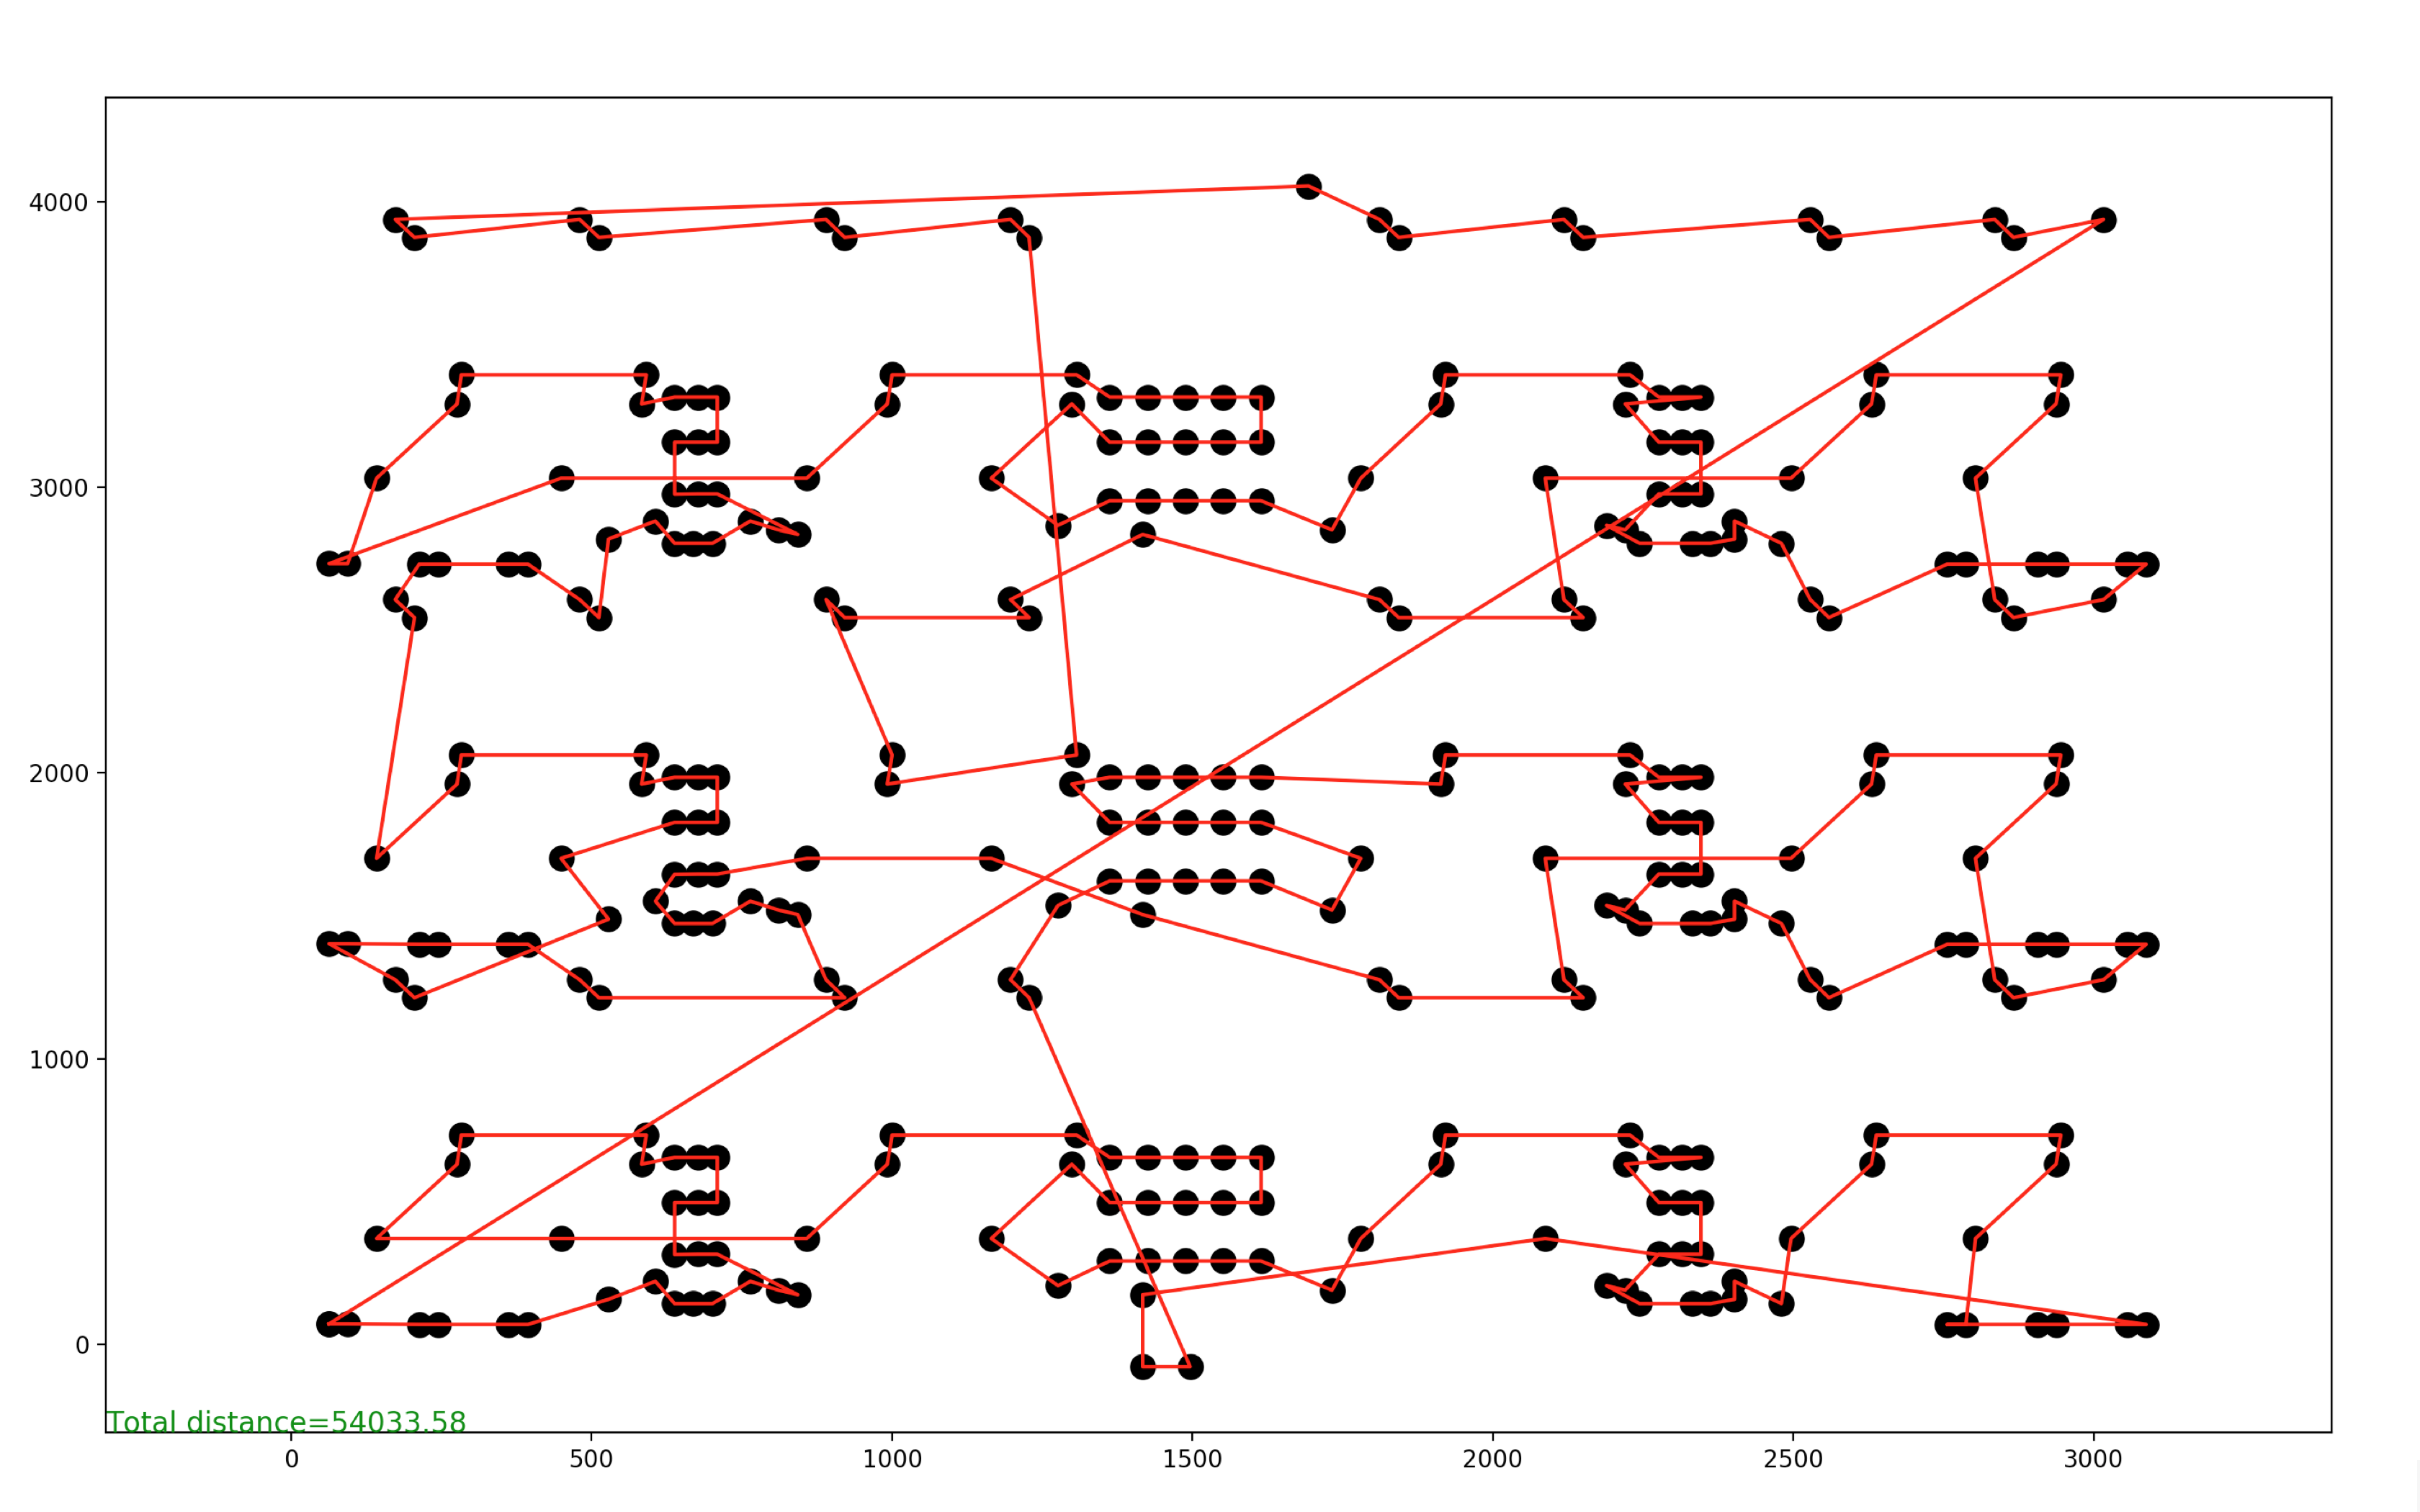
\includegraphics[width=1\textwidth]{../image/semipilot/semipilot-linhp318-2-2.png}
		\caption{\label{fig:Figura1} Tsp semipilot data linhp318}
	\end{minipage}
\end{figure}

\begin{table}[H]
\centering
\caption{Comparativa de tiempo de ejecución y distancia recorrida de Algoritmos para linhp318}
\label{Table:linhp318}
\begin{tabular}{| l | l | l | l |}
\hline
Algoritmo & Tiempo Inicial & Tiempo final & Distancia \\ \hline
Vecino más cercano & 2018-03-05 23:19:02.562361 & 2018-03-05 23:19:02.910580 & 54033.58 \\ \hline
Semi-pilot & 2018-03-05 23:21:31.198604 & 2018-03-05 23:21:31.767005 & 54033.58 \\ \hline
TSPLIB & - & - & 41345 \\ \hline

\end{tabular}
\end{table}

\subsection{Datos ch150}

\begin{figure}[H]
	\begin{minipage}{0.5\textwidth}
		\centering
		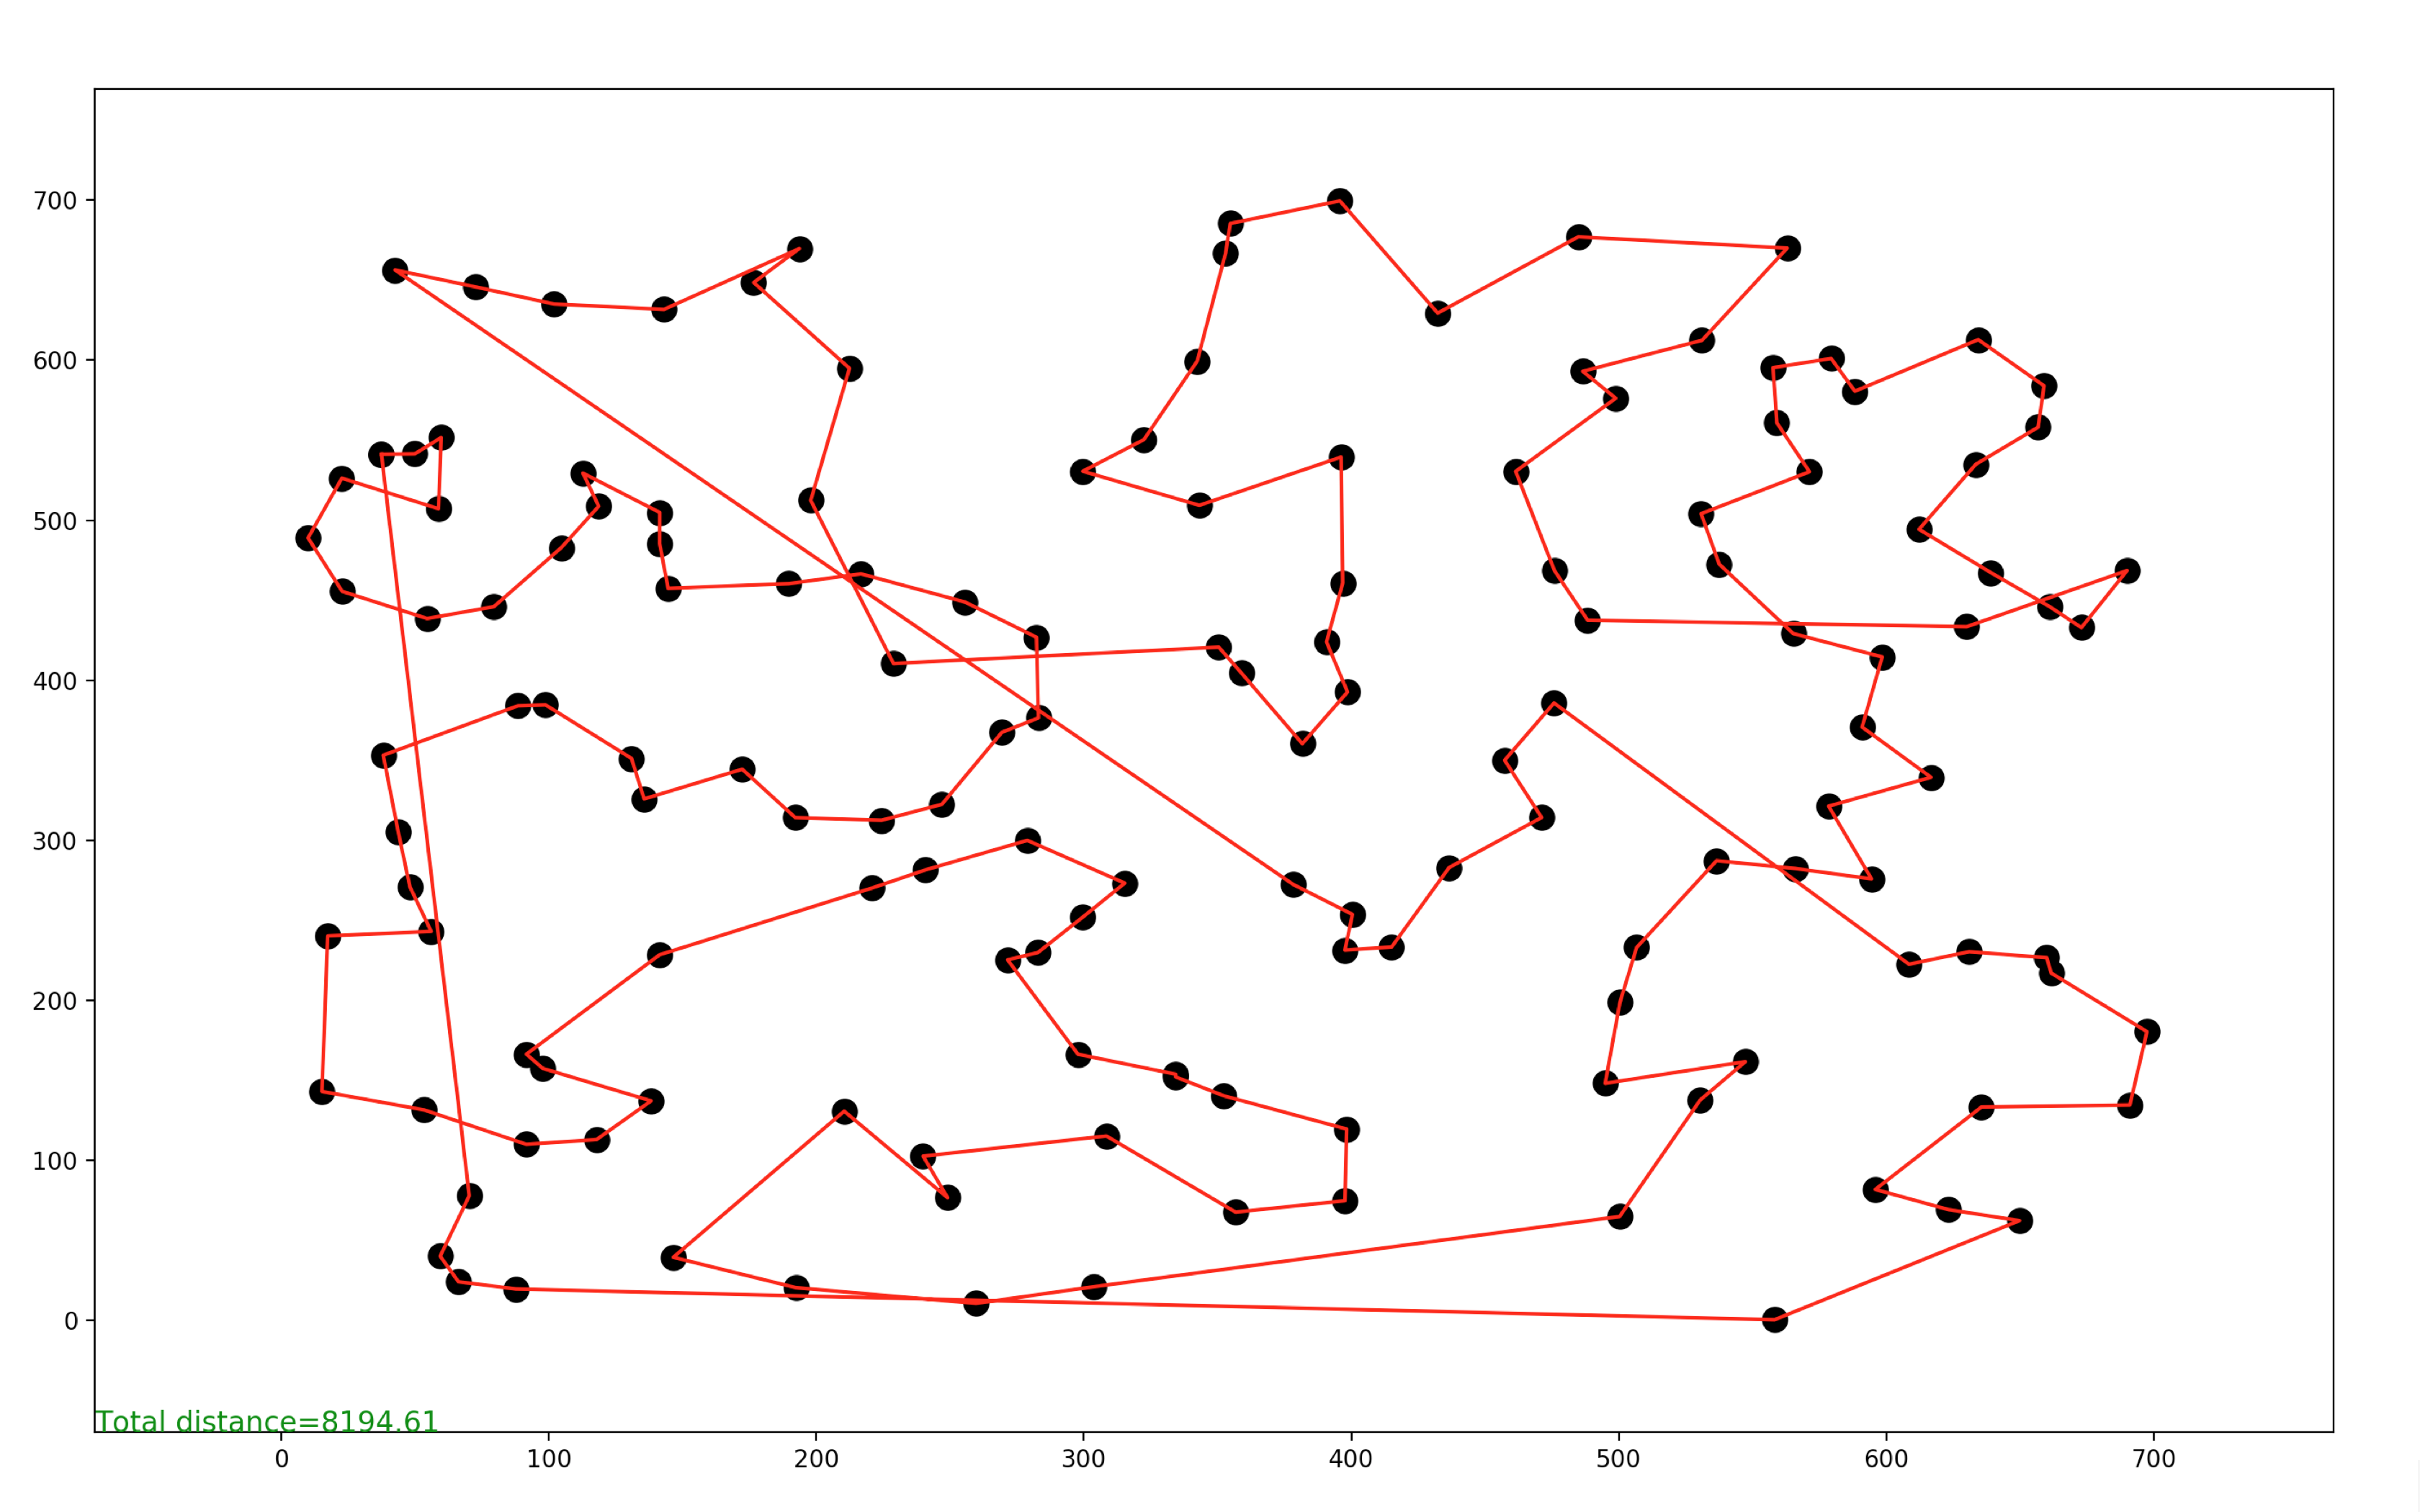
\includegraphics[width=1\textwidth]{../image/greedy/greedy-ch150.png}
		\caption{\label{fig:Figura1} Tsp greedy data ch150}
	\end{minipage}\hfill
	\begin {minipage}{0.5\textwidth}
		\centering
		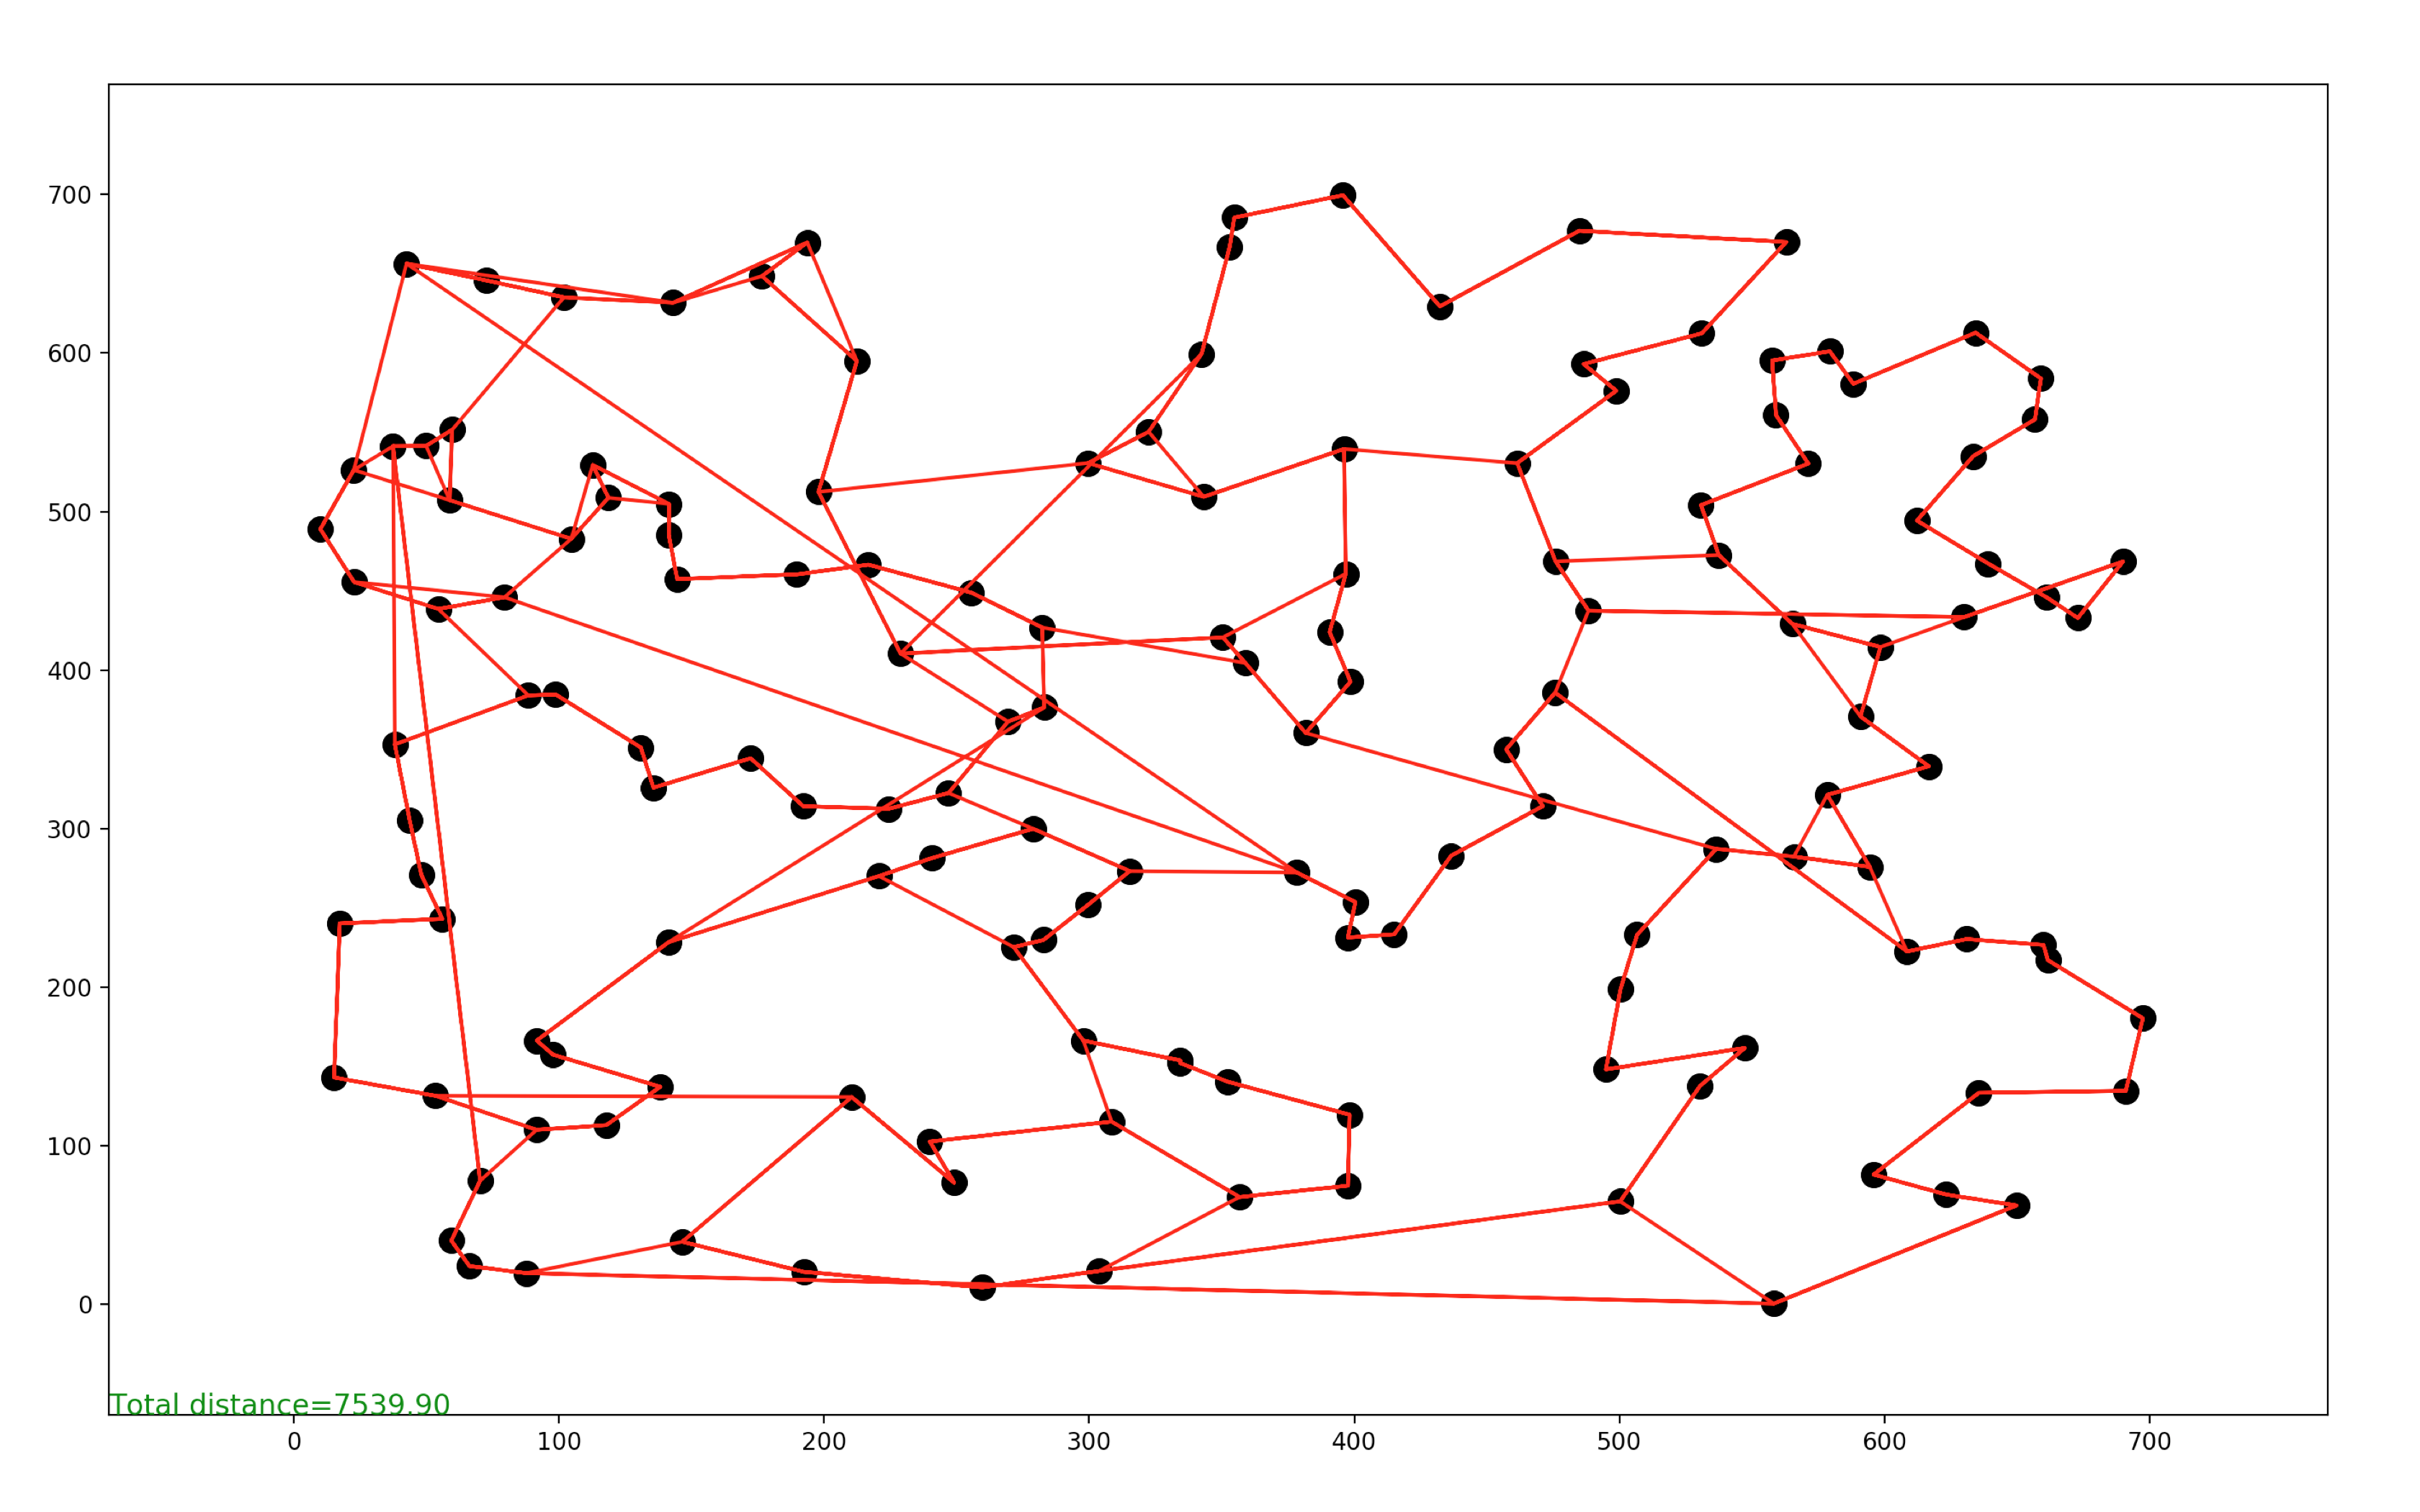
\includegraphics[width=1\textwidth]{../image/semipilot/semipilot-ch150-2-4.png}
		\caption{\label{fig:Figura1} Tsp semipilot data ch150}
	\end{minipage}
\end{figure}

\begin{table}[H]
\centering
\caption{Comparativa de tiempo de ejecución y distancia recorrida de Algoritmos para ch150}
\label{Table:ch150}
\begin{tabular}{| l | l | l | l |}
\hline
Algoritmo & Tiempo Inicial & Tiempo final & Distancia \\ \hline
Vecino más cercano & 2018-03-05 23:23:58.057231 & 2018-03-05 23:23:58.404496 & 8194.61 \\ \hline
Semi-pilot & 2018-03-05 23:24:53.177867 & 2018-03-05 23:24:53.578829 & 8145.80 \\ \hline
TSPLIB & - & - & 6528 \\ \hline

\end{tabular}
\end{table}

\subsection{Datos Berlin52}

\begin{figure}[H]
	\begin{minipage}{0.5\textwidth}
		\centering
		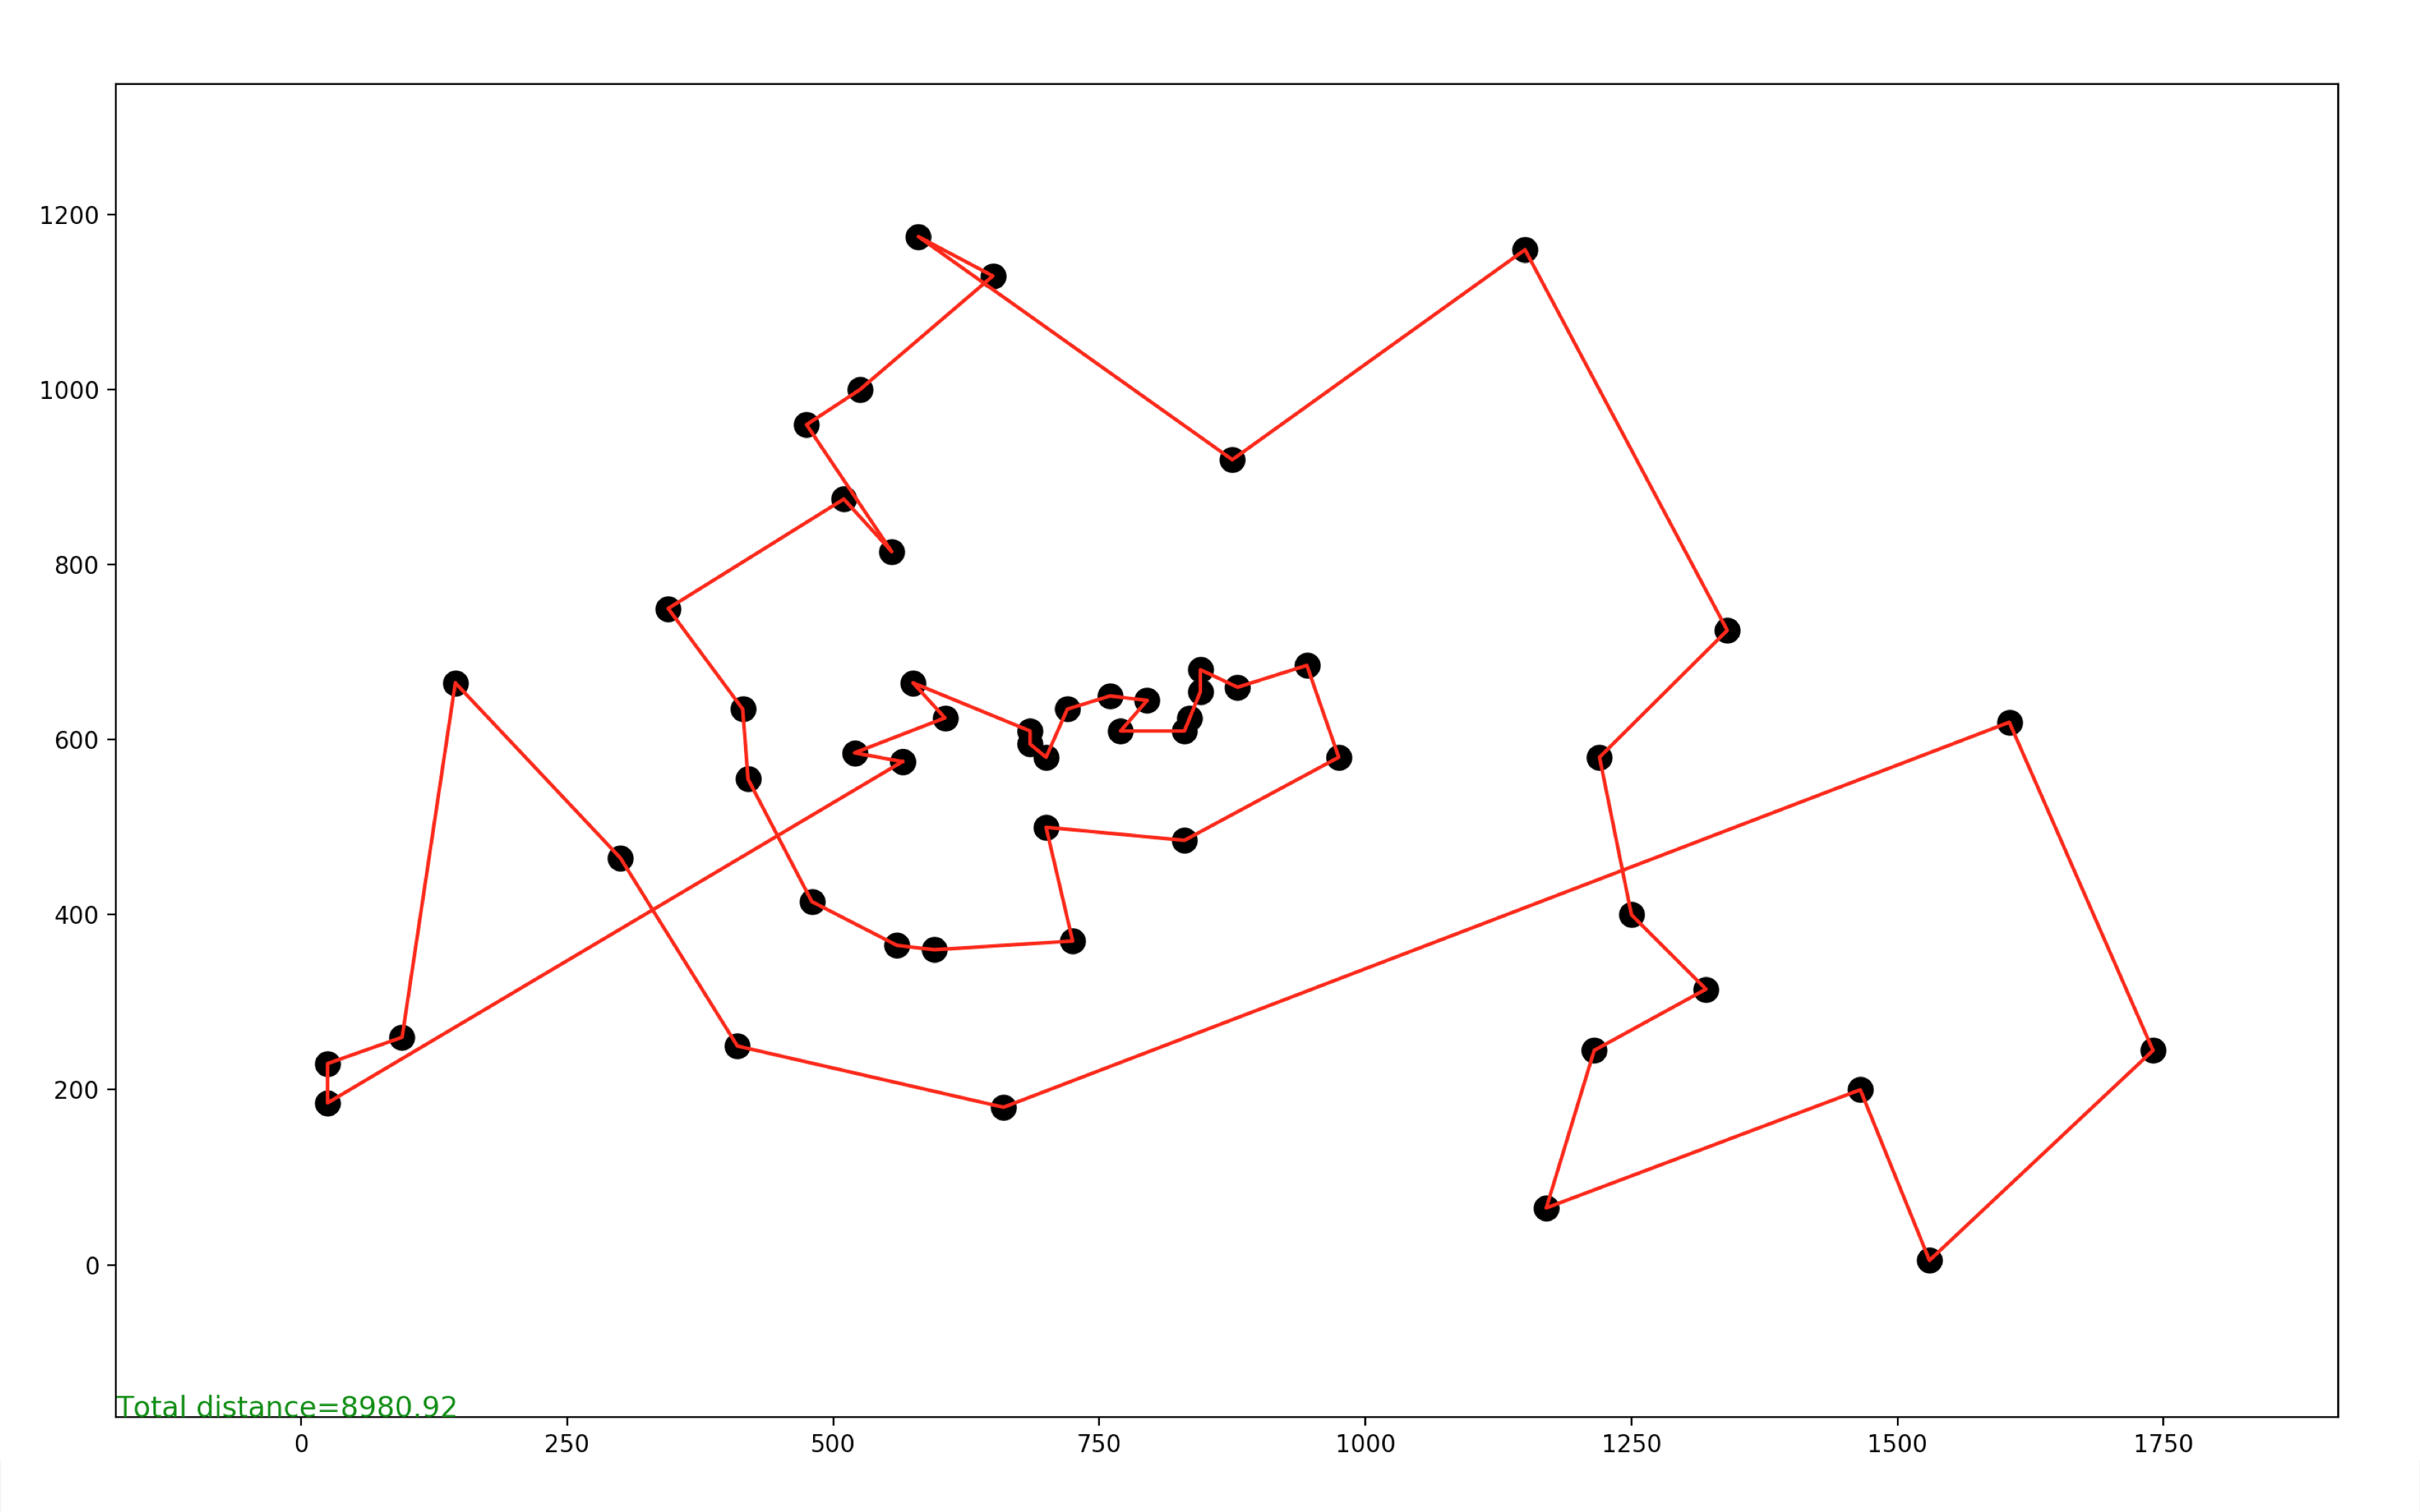
\includegraphics[width=1\textwidth]{../image/greedy/greedy-berlin52.png}
		\caption{\label{fig:Figura1} Tsp greedy data berlin52}
	\end{minipage}\hfill
	\begin {minipage}{0.5\textwidth}
		\centering
		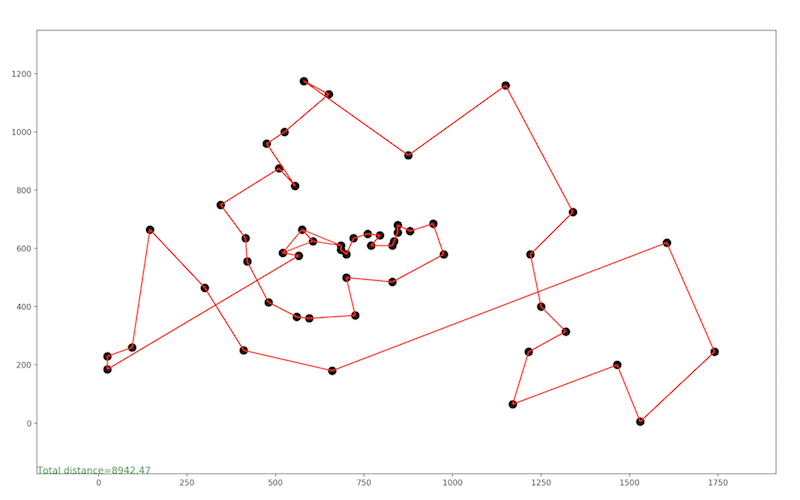
\includegraphics[width=1\textwidth]{../image/semipilot/semipilot-berlin52-2-2.png}
		\caption{\label{fig:Figura1} Tsp semipilot data berlin52}
	\end{minipage}
\end{figure}

\begin{table}[H]
\centering
\caption{Comparativa de tiempo de ejecución y distancia recorrida de Algoritmos para berlin52}
\label{Table:berlin52}
\begin{tabular}{| l | l | l | l |}
\hline
Algoritmo & Tiempo Inicial & Tiempo final & Distancia \\ \hline
Vecino más cercano & 2018-03-05 23:26:28.184412 & 2018-03-05 23:26:28.520302 & 8980.92 \\ \hline
Semi-pilot & 2018-03-05 23:27:14.091881 & 2018-03-05 23:27:14.421187 & 8942.47 \\ \hline
TSPLIB & - & - & 7542 \\ \hline

\end{tabular}
\end{table}

\section{Conclusiones}
\begin{itemize}
\item El método de semi-pilot para un pilot de 2 genera mejor solución que el método del vecino más cercano.
\item Los tiempos de ejecución son más extensos en el algoritmo semi-pilot, esto es debido a la evaluación de varios caminos.
\item El método semi-pilot para pilot muy grandes los tiempos de ejecución se elevan exponencialmente y las soluciones no mejoran significativamente.
\item El método del vecino más cercano es un algoritmo muy potente en relación a los tiempos de ejecución.
\item En los datos de linhp318 los dos algoritmos obtuvieron las mismas distancias lo que indica que la estrategia semi-pilot es vulnerable a ciertos patrones en las coordenadas.
\item Ambos algoritmos por la estrategia greedy que manejan son castigados al unir la coordenada final con la inicial.
\item Las implementaciones realizadas en TSPLIB superan significativamente a las soluciones construidas.
\end{itemize}

\end{document}
